\documentclass[english]{panikzettel}
\usepackage{amsthm}

\usepackage{listings}
\lstset{escapechar=\&,
        stringstyle=\ttfamily,
        keywordstyle=\bold,
        emph={Action, Precond, Effect, Op},
        emphstyle={\bfseries}
    }

\usepackage{nicefrac}

\usepackage{array}
\newcolumntype{L}{>{$}l<{$}}
\newcolumntype{C}{>{$}c<{$}}
\newcolumntype{R}{>{$}r<{$}}

\usepackage{tabularx}
\newcolumntype{P}{>{\raggedright\arraybackslash}X}

\usepackage{tikz}
\usetikzlibrary{shapes.multipart}
\usetikzlibrary{positioning}

\newcommand{\A}{\mathcal{A}}
\newcommand{\M}{\mathcal{M}}

\newcommand{\rk}{\mathrm{rk}}
\newcommand{\dom}{\mathrm{dom}}
\newcommand{\val}{\mathrm{val}}

\title{Advanced Automata Theory Panikzettel}
\author{Caspar Zecha, Tobias Polock, Philipp Schröer}

\begin{document}

\maketitle

\tableofcontents

\section{Introduction}

This Panikzettel is about the lecture Advanced Automata Theory by Prof.\ Löding held in the summer semester 2018.

This Panikzettel is Open Source. We appreciate comments and suggestions at \\ \url{https://git.rwth-aachen.de/philipp.schroer/panikzettel}.

\section{Notation and Automata}
We use the following notation in this lecture and define the basic automata:

\begin{halfboxl}
    \vspace{-\baselineskip}
    \begin{itemize}
        \item $\Sigma,\Gamma,\dots$ for alphabets,
        \item $a,b,\dots$ for letters,
        \item $\varepsilon$ for the empty word,
        \item $u,v,w,\dots$ for words,
    \end{itemize}
\end{halfboxl}%
\begin{halfboxr}
    \vspace{-\baselineskip}
    \begin{itemize}
        \item $\Sigma^*$ ($\Sigma^+$) for the set of words (of non-empty words) over $\Sigma$,
        \item $L,K,\dots$ for languages (subsets of $\Sigma^*$),
        \item $\mathcal{A},\mathcal{B},\dots$ for automata.
    \end{itemize}
\end{halfboxr}

\begin{halfboxl}
    \vspace{-\baselineskip}
    \begin{defi}{Nondeterministic Finite Automaton (NFA)}
        $\mathcal{A}=(Q,\Sigma,q_0,\Delta,F)$ with
        \begin{itemize}
            \item finite state set $Q$, initial state $q_0 \in Q$,
            \item transition relation $\Delta \subseteq Q \times \Sigma \times Q$,
            \item set $F \subseteq Q$ of final states.
        \end{itemize}

        $\mathcal{A}$ \emph{accepts} $w=a_1 \dots a_m$ if there is a \emph{run} $\varrho=\varrho(0) \dots \varrho(m)$ with $\varrho(m) \in F$ and
        \begin{tightcenter}
            $\varrho(0)=q_0$, $(\varrho(i-1),a_i,\varrho(i)) \in \Delta$.
        \end{tightcenter}

        The language recognised by $\mathcal{A}$ is
        \begin{tightcenter}
            $L(\mathcal{A}):=\{w \in \Sigma^* \mid \mathcal{A} \text{ accepts } w\}$.
        \end{tightcenter}
    \end{defi}
\end{halfboxl}%
\begin{halfboxr}
    \vspace{-\baselineskip}

    \begin{defi}{Deterministic Finite Automaton (DFA)}
        $\mathcal{A}=(Q,\Sigma,q_0,\delta,F)$ with
        \begin{itemize}
            \item finite state set $Q$, initial state $q_0 \in Q$,
            \item transition function $\delta : Q \times \Sigma \rightarrow Q$,
            \item set $F \subseteq Q$ of final states.
        \end{itemize}

        The language accepted by $\mathcal{A}$ is
        \begin{tightcenter}
            $L(\mathcal{A}):=\{w \in \Sigma^* \mid \delta^*(q_0,w) \in F \}$.
        \end{tightcenter}
        $\delta^* : Q \times \Sigma^* \rightarrow Q$ is defined as:
        \vspace{-\baselineskip}
        \begin{align*}
            \delta^*(q,\varepsilon) & := q,                       \\
            \delta^*(q,wa)          & := \delta(\delta^*(q,w),a).
        \end{align*}
    \end{defi}
\end{halfboxr}

We can create a DFA from an NFA recognising the same language by using subset construction.
Here the idea is to collect the NFA's non-deterministic possibilities as subsets, consisting of all reachable states from the previous subset.
The initial subset consists of only the initial state. Subset construction on an NFA with $n$ states may in worst case lead to a DFA with $2^n$ states.

\section{Minimisation of NFAs}
DFAs can be minimised by merging equivalent states.
The result is a unique minimal DFA that is equivalent to the given DFA.
This minimisation is efficient (polynomial time).

We want to analyse the problem of state merging on NFAs, i.e.\ taking the quotient of an automaton. Merging states can change the accepted language.

\subsection{Quotient Automaton}
Let $\mathcal{A}=(Q,\Sigma,q_0,\Delta,F)$ be an NFA and let $\sim$ be some \emph{equivalence relation} (reflexive, symmetric and transitive) on $Q$.
For a state $q \in Q$, the equivalence class is defined as $[q]_{\sim}=\Set{p \in Q \mid p \sim q}$.

Now the \emph{quotient automaton} $\mathcal{A}_{/\sim}$ of an NFA with respect to some equivalence relation $\sim$ is easy.
Merge states into equivalence classes (single states) and connect two classes if there exists a transition from a state of one class to a state in the other class.
A state representing an equivalence class is \emph{initial} or \emph{accepting} if at least one of the states it contains is.

By induction one can show that the quotient automaton accepts all words in $L(\mathcal{A})$ and an example can be given where the equivalence relation leads to $L(\mathcal{A}) \subset L(\mathcal{A}_{/\sim})$. Thus in general $L(\mathcal{A}) \subseteq L(\mathcal{A}_{/\sim})$. To assure that the language is not changed consider only relations which merge language equivalent states.

\subsubsection{Quotient on DFAs}
Viewing a DFA as an NFA and then applying the quotient operation on the NFA, the resulting quotient $\mathcal{A}_{/\sim}$ is a DFA again exactly if $\sim$ is a \emph{congruence relation} w.r.t.\ the transition function $\delta$: $p \sim q \implies \delta(p,a) \sim \delta(q,a) \Forall a \in \Sigma$.

For DFA $\mathcal{A}$ and $q \in Q$, let $\mathcal{A}_q$ be the DFA $\mathcal{A}$ with $q$ as initial state.
We then define $\sim_\mathcal{A}$ by $q \sim_\mathcal{A} p$ iff $L(\mathcal{A}_q) = L(\mathcal{A}_p)$ and call states $q$ and $p$ \emph{language equivalent}.

Using this, the quotient $\mathcal{A}_{/\sim_\mathcal{A}}$ is the \emph{minimal DFA accepting the same language as $\mathcal{A}$}.
The minimal DFA can be computed efficiently in $\mathcal{O}(|\Sigma||Q| \cdot \log |Q|)$.

\subsection{Reduction of NFAs}

\begin{halfboxl}
    Minimal NFAs can be exponentially smaller than minimal DFAs w.r.t.\ the number of states.
    However, there can be several non-isomorphic minimal NFAs for a language.

    Additionally, deciding whether an NFA is minimal is computationally hard (PSPACE-complete), as are the two other decision problems on the right.
    Remember: P $\subseteq$ NP $\subseteq$ PSPACE.
\end{halfboxl}%
\begin{halfboxr}
    \vspace{-\baselineskip}
    \begin{defi}{NFA Decision Problems}
        Given NFAs $\mathcal{A}$, $\mathcal{B}$ over the same alphabet.

        \begin{enumerate}
            \item  Is $\mathcal{B}$ an NFA equivalent to $\mathcal{A}$ with the least possible number of states?
            \item Are $\mathcal{A}$ and $\mathcal{B}$ equivalent?
            \item Is $L(A) \neq \Sigma^*$? (minimal NFA has more than one state)
        \end{enumerate}
    \end{defi}
\end{halfboxr}

%The proof in the lecture demonstrates PSPACE-completeness by providing a polynomial-time reduction for every language $D$ in PSPACE to the NFA non-universality problem (problem 3).

%The proof constructs, from a PSPACE-bounded TM $M$, an NFA.
%The NFA only rejects an accepting computation of $M$ by searching for an error in the input word.
%Because of the space bound, the NFA can compare a position in a configuration with the same position in the successive configuration (by counting the number of steps to get there from the start of the configuration in the state). To be constructed in polynomial time, the NFA guesses where the error occurs.

\subsection{Bisimulation}

\begin{halfboxl}
    \emph{Bisimulation} provides an equivalence relation on the states of an NFA.
    It is similar to the $\sim_\mathcal{A}$ relation for DFAs.

    The bisimulation relation $\approx_\mathcal{A}$ is the biggest relation (w.r.t.\ $\subseteq$) that satisfies the following three conditions:
    If $p \approx_{\mathcal{A}} q$, then
    \begin{itemize}
        \item $p \in F \Leftrightarrow q \in F$,
        \item $\Forall (p,a,p') \in \Delta \Exists (q,a,q') \in \Delta: p' \approx_\mathcal{A} q'$,
        \item $\Forall (q,a,q') \in \Delta \Exists (p,a,p') \in \Delta: p' \approx_\mathcal{A} q'$.
    \end{itemize}

    This relation can also be characterised as the \emph{bisimulation game} (see right).
    If the Duplicator has a winning strategy in $\text{BG}(\mathcal{A},p,\mathcal{B},q)$, we call $(\mathcal{A}, p)$ and $(\mathcal{B},q)$ bisimilar.
    \medskip
    \begin{tightcenter}$p \approx_\mathcal{A} q \iff (\mathcal{A},p) \approx (\mathcal{A},q)$\end{tightcenter}
\end{halfboxl}%
\begin{halfboxr}
    \vspace{-\baselineskip}
    \begin{defi}{Bisimulation Game}
        Given two automata $\mathcal{A},\mathcal{B}$ with $p \in Q_{\mathcal{A}}$ and $q \in Q_{\mathcal{B}}$, we denote the bisimulation game between the \textit{spoiler} and the \textit{duplicator} as
        \[\text{BG}(\mathcal{A},p,\mathcal{B},q).\]

        From a configuration $(p',q')$ the spoiler chooses a transition $(p',a,p'') \in \Delta_{\mathcal{A}}$ or $(q',a,q'') \in \Delta_{\mathcal{B}}$.

        Then the duplicator reacts accordingly from the other state.

        Unless the spoiler creates a configuration $(\Tilde{p},\Tilde{q})$ such that $\Tilde{p} \in F_{\mathcal{A}} \Leftrightarrow \Tilde{q} \not \in F_{\mathcal{B}}$ or the duplicator doesn't have a transition over the chosen letter, the duplicator wins.
    \end{defi}
\end{halfboxr}

\subsection{Block Refinement}

\begin{halfboxl}
    We can compute the bisimulation equivalence using \emph{block refinement}.
    This algorithm iteratively tries to split \emph{blocks} of states until they cannot be separated by words anymore.

    When the blocks can be split, they're called \emph{not compatible}: If there are $p,q \in B$ with
    \begin{itemize}
        \item $\Exists (p,a,p') \in \Delta$ with $p' \in B'$
        \item $\neg \Exists (q,a,q') \in \Delta$ with $q' \in B'$
    \end{itemize}

    The algorithm's complexity is $O(\abs{\Delta} \cdot \abs{Q})$.
\end{halfboxl}%
\begin{halfboxr}
    \vspace{-\baselineskip}
    \begin{algo}{Block Refinement}
        \textbf{Input:} NFA $\mathcal{A} = (Q, \Sigma, q_0, \Delta, F)$.

        \textbf{Output:} Partition $\pi$.
        \tcblower
        \begin{enumerate}
            \item $\pi = \Set{ Q \setminus F, F }$.
            \item While $\Exists B, B' \in \pi, a \in \Sigma$ such that $B \text{ is not compatible with } (B',a)$:
                \begin{itemize}
                    \item split $B$ with respect to $(B',a)$ into \\
                            $\Set{p \in B | \Exists p' \in B' : (p,a,p') \in \Delta}$, \\
                            $\Set{p \in B | \neg \Exists p' \in B' : (p,a,p') \in \Delta}$.
                \end{itemize}
        \end{enumerate}
    \end{algo}
\end{halfboxr}

\subsection{Comparison of Reductions}
Thus the $\approx_\mathcal{A}$-quotient can be bigger than the $\sim_\mathcal{A}$-quotient.
The latter can be bigger than the \emph{optimal quotient} (the smallest quotient NFA that accepts the same language as $\mathcal{A}$).
But the optimal quotient is not necessarily the smallest equivalent NFA, imagine for example an NFA that does not use its non-determinism: its quotient automaton can not be smaller than the minimal DFA.

\section{Learning Algorithms for DFAs}
We want to develop an algorithm (\emph{learner}) that constructs a \emph{deterministic} finite automaton for an unknown language $L$.
The learner has some information about $L$.
Different settings are possible:
\begin{itemize}
    \item \emph{Passive}: The learner is given a finite set of words (not) in $L$.
    \item \emph{Active}: The learner can query the language. They can ask whether a word $w$ is in L or can construct an automaton $\mathcal{A}$ and ask whether $L=L(\mathcal{A})$.
\end{itemize}

\subsection{Passive: Construction of Finite Automata from Examples}

\begin{halfboxl}
    We first consider the passive learning where we want learners as computable functions $f$ that take a sample $S$ and return a DFA $\mathcal{A} = f(S)$.

    The learner should be \emph{consistent}, that is $f(S)$ should be consistent with every sample $S$.
    But this is not enough, as a simple consistent learner may not generalise well -- e.g.\ accepting precisely the given samples, but not more.

    Therefore we define $f$ \emph{learning in the limit} if there is an $n_0$ such that for all $n \geq n_0: L(f(S^{L,n})) = L$.

    The set of positive (negative) samples contains all words that are lexicographically smaller than the $n$th word and (not) in the language $L$.
\end{halfboxl}%
\begin{halfboxr}
    \vspace{-\baselineskip}
    \begin{defi}{Sample}
        \emph{Samples} are of the form $S=(S_+,S_-)$ where $S_+$ ($S_-$) is a finite set of positive (negative) examples where $S_+ \cap S_- = \emptyset$.

        A DFA $\mathcal{A}$ is \emph{consistent} with $S$ if $S_+ \subseteq L(\mathcal{A})$ and $S_- \cap L(\mathcal{A})=\emptyset$.
    \end{defi}

    \vspace{-\baselineskip}
    \begin{align*}
        S^{L,n}_+ &= \Set{w_i \in L | i \leq n} \\
        S^{L,n}_- &= \Set{w_i \notin L | i \leq n} \\
        S^{L,n} &= (S^{L,n}_+, S^{L,n}_-)
    \end{align*}
\end{halfboxr}

Let $f$ be a learner such that $f(S)$ is a smallest DFA that s consistent with $S$, for each sample $S$.
Then, $f$ learns all regular languages in the limit.
There exists a learner that constructs a smallest DFA that is consistent for each sample $S$.
The learner enumerates all DFAs by increasing size and checks for consistency with $S$.

Unfortunately, checking whether there exists a DFA with at most $m$ states that is consistent with a sample $S$ is NP-complete.
This can be shown using a reduction from the 3-Coloring decision problem which translates to the question "Is there a consistent DFA with at most 4 states?", encoding adjacency constraints of the coloring problem in the negative samples and using positive samples to simulate coloring.

\newpage
\subsection{Regular Positive Negative Inference (RPNI)}

The \emph{RPNI-algorithm} is a learner that computes a DFA $f(S)$ for a sample $S$ in polynomial time and learns every regular language in the limit.

The algorithm first constructs a simple ``prefix tree acceptor'' DFA $\A(S_+)$ which accepts exactly all words from $S_+$.
Then the automaton is simplified using quotients with regard to congruence relations.
The quotients are tried in canonical order, and only those that are consistent with the sample are used.
Thus the automaton is simplified and its language is generalised, i.e.\ $S_+$ is still accepted, and $S_-$ is still rejected.

\begin{algo}{Regular Positive Negative Inference (RPNI)}
    \textbf{Input}: Sample $S = (S_+, S_-)$.

    \textbf{Output}: (partial) DFA $\mathcal{A}(S_+)_{/\sim}$.
    \tcblower
    \begin{enumerate}
        \item Construct $\A(S_+)$ accepting precisely $S_+$.
        (States are prefixes of words in $S_+$)
        \item Sort states $Q_+ = \Set{ u_0, \ldots, u_n }$ from $\A(S_+)$ in \emph{canonical order}:
            \begin{tightcenter}
                $u < v \iff \abs{u} < \abs{v} \lor (\abs{u} = \abs{v} \land u \text{ is before } v \text{ in lexicographic ordering})$.
            \end{tightcenter}
        \item Initialise $\sim ~= \Set{ (u,u) | u \in Q_+ }$. \\
            {\footnotesize{}\textcolor{darkgray}{$\A(S_+)_{/\sim}$ looks just like $\A(S_+)$.}}
            \smallskip
        \item For each $u_i \in Q_+ \setminus \Set{u_0}$:
            \smallskip
            \begin{itemize}
                \item If $u_i \not\sim u_j$ for all $u_j \in \Set{ u_0, \ldots, u_{i-1} }$: \\
                    {\footnotesize{}\textcolor{darkgray}{Skip words that have already been merged with smaller words (in canonical order)}}
                    \smallskip
                    \begin{itemize}
                        \item Try next $u_k \in Q_+$ with $k < i$, until $L(\A(S_+)_{/\sim'}) \cap S_- \neq \emptyset$. \\
                            {\footnotesize{}\textcolor{darkgray}{Try to merge with the next (smaller) state (in canonical order) such that no negative example is accepted.}}
                            \smallskip
                            \begin{itemize}
                                \item $\sim'$ = extend $\sim$ to the smallest congruence with $(u_i, u_k)$. \\
                                    {\footnotesize{}\textcolor{darkgray}{Merge states containing $u_i$ and $u_k$ and preserve congruence, i.e.\ if merging creates transitions to different states in the quotient, recursively merge those too.}}
                                    \smallskip
                            \end{itemize}
                        \item Commit $\sim ~=~ \sim'$.
                    \end{itemize}
            \end{itemize}
    \end{enumerate}
\end{algo}

We consider the question ``When is a sample complete enough for RPNI to produce a DFA for $L$?''

First we need \emph{minimal representatives} and \emph{minimal transition representatives} for $L$:
\begin{align*}
    \mathrm{MR}(L) &:= \Set{ w \in \Sigma^\ast | w \in prf(L) \land \Forall u \sim_L w: w \leq u } \\
    \mathrm{MTR}(L) &:= \Set{ w \in \Sigma^\ast |
        \begin{array}{c}
            w \in prf(L) \land w = ua \\
            u \in \mathrm{MR}(L) \land a \in \Sigma
        \end{array}
    }
\end{align*}

We define a sample $S$ \emph{RPNI-complete for $L$} if
\begin{itemize}
    \item For each $q \in F_L$ ($F_L$ being the final states in the minimal automaton for $L$), there is a $u \in S_+$ such that $u$ reaches $q$ in $\A_L$,
    \item $\Forall w \in \mathrm{MTR}(L)$, there is a $v \in \Sigma^\ast$ such that $wv \in S_+$,
    \item $\Forall u \in \mathrm{MR}(L)$ and $\Forall v \in \mathrm{MTR}(L)$ with $u \not\sim_L v$, there exists a $w$ such that $uw, vw \in S$ and $uw \in S_+ \iff vw \in S_-$.
\end{itemize}

If a sample is RPNI-complete, then RPNI will compute the minimal DFA for the language.
For each regular language $L$, there is a RPNI-complete sample of polynomial size in the size of $\A_L$.

\subsection[Active Learning with L*]{Active Learning with $L^\ast$}

In active learning the learner can ask specific questions about the target language.
We consider the \emph{Minimally Adequate Teacher (MAT) model} which has the following two types of questions:
\begin{itemize}
    \item Membership queries: ``Is $w \in L$?'' for a chosen word $w$.
    \item Equivalence queries: ``Does $\A$ accept $L$?'' for a DFA $\A$. \\
            If the answer is ``no'', then the teacher provides an arbitrary counter-example $w$.
\end{itemize}

The $L^\ast$ algorithm asks these queries to build a minimal DFA for the target language.
It does so indirectly by inferring $\sim_L$-classes, which correspond to states in $\A_L$.

The general idea is as follows:
We have a set of \emph{representatives} $R \subseteq \Sigma^\ast$ for our equivalence classes and a set of words, called \emph{experiments} $E \subseteq \Sigma^\ast$.
We've found a new representative $u \in R \cdot \Sigma$ if $u$ is \emph{escaping}: For all other representatives $v \in R$ there is an experiment $w \in E$, so that $uw \in L \Leftrightarrow vw \notin L$.
One can think of $u$ and the $v$s as states in the automaton: If starting from state $u$ we get a different result reading $w$ than starting from all $v$s, $u$ must be a distinct state.

If $u$ is not escaping, there is a unique representative $v \in R$ with $uw \in L \iff vw \in L$ for all experiments $w \in E$.
Then $u$ and $v$ are called \emph{compatible}.

\begin{minipage}[t]{0.82\textwidth}
    All our measurements are saved in an \emph{observation table} $B = (R, E, f)$ with representatives $R$, experiments $E$ and the data provided by a function
    $f : (R \cdot E \cup R \cdot \Sigma \cdot E) \to \Set{0,1}$.
    $B$ is an observation table for $L$ if $f(w) = 1 \Leftrightarrow w \in L$.

    In the top part, we have the $R \cdot E$.
    Throughout the algorithm, rows in the top are all distinct -- each row corresponds to one equivalence class.
    The bottom part contains all other measurements.
    Iff a row in the bottom is unique among all others, then the corresponding $w \in R \cdot \Sigma$ is escaping and we make it a representative (move it to the top).
    $B$ is \emph{closed} if no escaping $w \in R \cdot \Sigma$ exists.
\end{minipage}\hfill%
\begin{minipage}[t]{0.15\textwidth}
    \vspace{-\baselineskip}
    \begin{tightcenter}
        \begin{tabular}{|R|C|C|}
            B & \varepsilon & a  \\
            \hline \hline
            \varepsilon & 0 & 1 \\
            a & 1 & 1 \\
            ab & 0 & 0 \\
            \hline
            b & 1 & 1 \\
            aa & 1 & 1 \\
            aba & 0 & 0 \\
            abb & 1 & 1 \\
            \hline
        \end{tabular}
    \end{tightcenter}
\end{minipage}

After adding escaping words from $R \cdot \Sigma$ until $B$ is closed, we construct the \emph{hypothesis} $\A_B$ and ask the teacher the equivalence query.
The construction of the automaton is simple: Each of the representatives becomes a state, and each transition from a state $u \in R$ with $a$ goes to the unique $v \in R$ compatible with the word $ua$. Representative $\varepsilon$ becomes the initial state. Final states are all states with their representative $u \in R$ evaluating to 1, i.e $f(u \cdot \varepsilon) = 1$ in the observation table. 

If the hypothesis is correct, we're done.
Otherwise, we extend the experiments $E$ based on the counter-example $w = a_1 \cdots a_m$ the teacher provided.
First, define $r_i = \delta_B^\ast(q_0^B,a_1 \cdots a_i)$ to be the state reached in $\A_B$ after reading the prefix of length $i$ of $w$.
Per construction of $\A_B$, this is always a representative: $r_i \in R$.

Now we search for a \emph{breakpoint} $i \in \Set{1, \ldots, m}$ where our hypothesis automaton becomes wrong: $r_{i-1} a_i \cdots a_m \in L \iff r_i a_{i+1} \cdots a_m \notin L$.
We then add the remaining suffix $a_{i+1} \cdots a_m$ to our experiments $E$.
This makes $r_{i-1} a_i$ an escaping word and we must add it to $R$, introducing a new state in our hypothesis.

\begin{algo}{$L^\ast$}
    \textbf{Input}: Teacher $T$ for a regular language $L\in \Sigma^\ast$.

    \textbf{Output}: DFA $\mathcal{A}_B$.
    \tcblower
    \begin{itemize}
        \item Initialise $B=(R,E,f)$ with $R = \Set{\varepsilon}$, $E =\Set{\varepsilon}$ and $f(w) = T(w) \quad\Forall w \in \Set{\varepsilon} \cup \Sigma$.
        \item Repeat:
            \begin{enumerate}
                \item Add escaping words from $R \Sigma$ to $R$ until $B$ is closed, and fill the table.
                \item Ask an equivalence query for hypothesis $\A_B = (Q_B, \Sigma, q_0^B, \delta_B, F_B)$ with:
                    \begin{tightcenter}
                        $Q_B = R$, \quad $q_0^B = \varepsilon$, \quad $F_B = \Set{u | f(u) = 1}$, and \\
                        $\delta_B(u,a) = v$ for the (unique) $v \in R$ compatible with $ua$.
                    \end{tightcenter}
                \item If the hypothesis is correct, \texttt{return $\A_B$}.
                \item For a counter-example $W = a_1 \cdots a_m$:
                    \begin{enumerate}
                        \item Find a breakpoint $i$.
                        \item Add $a_{i+1} \cdots a_m$ to $E$ and fill the table.
                    \end{enumerate}
            \end{enumerate}
    \end{itemize}
\end{algo}

The algorithm $L^\ast$ terminates in polynomial time and returns a DFA $\A_B$ that is isomorphic to $\A_L$.

Each iteration of the loop increases $\abs{R}$, which is bounded by the index of $L$, since the representatives are all in different $\sim_L$-classes, separated by the experiments.

\section{Automata and Logic}

We want to decide whether all executions of a given transition system (automaton) satisfy a certain specification.
Therefore, we want a logic that is equivalent to automata in expressive power.

\subsection{MSO Logic on Words}

\begin{halfboxl}
    \vspace{-\baselineskip}
    \begin{defi}{Word Structure}
        A non-empty word $w = b_1 \dots b_m$ over $\Sigma = \Set{ a_1, \dots, a_n }$ defines the \emph{word structure}
        \begin{center}
            \footnotesize
            $\underline{w}=(dom(w), S^w, <^w, min^w, max^w, P^w_{a_1}, \dots, P^w_{a_n})$,
        \end{center}
        where
        \begin{itemize}
            \item $dom(w) = \Set{ 1, \dots, m }$ are positions,
            \item $S^w$ is the successor relation,
            \item $<^w$ the less relation on $dom(w)$,
            \item $min^w=1$ and $max^w=m$ and
            \item $P^w_{a_i}:= \Set{ j \in dom(w) \mid b_j = a_i }$ for $i = 1, \ldots, n$.
        \end{itemize}
    \end{defi}

    Note that we can eliminate $min$, $max$ and $S$ in FO and MSO, and in MSO $<$ instead of $S$.
\end{halfboxl}%
\begin{halfboxr}
    \vspace{-\baselineskip}
    \begin{defi}{Syntax of MSO Formulae}
        \centering
        \textsc{Variables} \\
        $x,~y,~z$ for positions, \\
        $X,~Y,~Z$ for sets of positions.

        \textsc{Constants} \\
        $min$, $max$

        \textsc{Atomic formulae} \\
        \begin{tabular}{Cc}
            x = y & \emph{equality} \\
            S(x,y) & \emph{successor} \\
            x < y & \emph{before} \\
            P_a(x) & \emph{$a$ at position $x$} \\
            X(y) & $y \in X$
        \end{tabular}

        \textsc{Complex formulae} \\
        with $\neg$, $\lor$, $\land$, $\rightarrow$, $\leftrightarrow$ and $\Exists$, $\Forall$.
    \end{defi}
\end{halfboxr}

We use \emph{monadic second-order} (MSO) logic.
This logic is a second-order logic with quantification over unary predicates.
We are allowed to quantify over sets!
Given an alphabet $\Sigma$, we have \emph{$MSO_\Sigma[S,<]$ formulae}.
Such formulae which only use quantifiers over first-order variables (position variables) are called \emph{$FO_\Sigma[S,<]$ formulae}.
If there are free variables of a formula $\varphi$ among $x_1, \dots, x_m,X_1, \dots, X_n$, then this is indicated by $\varphi(x_1, \dots, x_m,X_1, \dots, X_n)$.
A \emph{sentence} is a formula without free variables.


\begin{defi}{Interpretation of Formulae}
    \begin{minipage}[c]{0.6\textwidth}
        If $\varphi$ evaluates to true in $\underline{w}$ when interpreting $x_i$ by $k_i$ and $X_i$ by $K_i$:
        \begin{align*}
            (\underline{w}, k_1, \dots, k_m, K_1, \dots, K_n) &\models \varphi(x_1, \dots, x_m, X_1, \dots, X_n) \\
            \text{or} \quad\quad\underline{w} &\models \varphi[k_1, \dots, k_m, K_1, \dots, K_n]
        \end{align*}
    \end{minipage}\hfill%
    \begin{minipage}[c]{0.4\textwidth}
        \begin{itemize}
            \item $\underline{w}$ a word structure,
            \item $k_1, \dots, k_m$ positions $w$,
            \item $K_1, \dots, K_n$ sets of positions in $w$.
        \end{itemize}
    \end{minipage}
\end{defi}

The \emph{language defined by $\varphi$} is
$$L(\varphi) := \Set{ w \in \Sigma^+ | \underline{w} \models \varphi }.$$
If $\varphi$ is an $MSO_\Sigma[S,<]$-sentence, we call the language \emph{$MSO_\Sigma[S,<]$-definable} (MSO-definable for short).
If $\varphi$ does not use set quantifiers, then the language is called \emph{$FO_\Sigma[S,<]$-definable} (FO-definable for short).

\subsection{The Equivalence Theorem}

We show the equivalence of automata and formulae. In the direction from automata to formulae we build a formula that expresses the existence of an accepting run in the automaton. In the other direction from formulae to automata we use induction over the structure of the formula.

\begin{theo}{Equivalence Theorem}
A language $L \in \Sigma^*$ is regular iff it is MSO-definable.
\end{theo}

\subsubsection{From Automata to Formulae}

We want to construct a sentence $\varphi_\A$ with $\underline{w} \models \varphi_\A \text{ iff } w \in L(\A)$.
$\varphi_\A$ has to express that there is an accepting run of the NFA $\A$ on $w$.

The idea is to ask for $i$ sets $X_i$, one for each state, where $X_i$ is the set of positions in which $\A$ is in state $i$.

Let $\A=(\{1,\dots,m \}, \Sigma, 1, \Delta, F)$ be an NFA. $\A$ accepts $w$ iff $\underline{w} \models \varphi_\A$.

\begin{tabular}{Lr}
    \varphi_\A := \exists X_1,\dots \exists X_m [ &  \\
    \hspace{1em} \hphantom{\land} \forall x (X_1(x) \lor \dots \lor X_m(x)) \land \bigwedge_{i \neq j} \neg \exists x (X_i(x) \land X_j(x)) & \footnotesize{($X_1, \ldots, X_m$ form a partition)} \\
    \hspace{1em} \land X_1(min) & \footnotesize{(on min, the initial state is used)} \\
    \hspace{1em} \land \forall x\forall y ( S(x,y) \rightarrow \bigvee_{(i,a,j) \in \Delta} (X_i(x) \land P_a(x) \land X_j(y))) & \footnotesize{(transitions are used everywhere)} \\
    \hspace{1em} \land \bigvee{(i,a,j) \in \Delta,j \in F} (X_i(max) \land P_a(max)) & \footnotesize{(last transition goes to an accepting state)} \\
    ]
\end{tabular}

\subsubsection{From Formulae to Automata}

We construct the automaton inductively over the structure over the formulae.
Since automata are closed over negation, intersection and union, translation of $\neg$, $\land$ and $\lor$ is easy.
However, variables are more difficult.

\begin{halfboxl}
    We first translate the formulae to MSO$_0$, which is a subset of MSO-formulae where all variables are set variables (the usual first-order variables are replaced).
    The idea here is to use singleton sets $\Set{x}$ for all first-order variables $x$.

    \begin{theo}{MSO$_0$ Equivalence}
        Each MSO sentence $\varphi$ over words is equivalent to an MSO$_0$ sentence.
    \end{theo}
\end{halfboxl}%
\begin{halfboxr}
    \vspace{-\baselineskip}
    \begin{defi}{Syntax of MSO$_0$}
        \centering
        Like MSO, but only with set variables and:

        \textsc{Atomic formulae} \\
        \begin{tabular}{Cc}
            X \subseteq Y & \emph{subset} \\
            X \subseteq P_a & \emph{only positions of $a$} \\
            Sing(X) & $\abs{X} = 1$ \\
            S(X,Y) & {\footnotesize{}$X = \Set{x}, Y = \Set{y}$,} $S(x,y)$ \\
            X < Y & {\footnotesize{}$X = \Set{x}, Y = \Set{y}$,} $x < y$
        \end{tabular}
    \end{defi}
\end{halfboxr}
\vspace{-0.5\baselineskip}

One can specify an automaton for each MSO$_0$ formula inductively over the syntax of such formulae.
For simplicity, we restrict formulae to operators $\land, \neg$ and existential quantifiers.
For MSO$_0$ formulae over $\Sigma$ with $n$ free variables, the automaton will recognise a language over the alphabet $\Sigma \times \Set{0,1}^n$.
The $\Set{0,1}^n$ part encodes membership of positions of the free (set-)variables $X_1,\ldots,X_n$.
Note that while words are defined over sentences (no free variables), an inductive definition requires handling formulae with free variables that arise in sub-formulae of quantors.

For the translation, assume prenex normal form, that is
\begin{tightcenter}
    $Q_1 X_1~ \ldots Q_n X_n~ \eta(X_1, \ldots, X_n)$ with $Q_i \in \Set{ \Forall, \Exists }$, $\eta$ is quantifier-free.
\end{tightcenter}
In the following we denote bitvectors in $\Sigma \times \Set{0,1}^n$ as $(a, x_1,\ldots,x_n)$.

{\renewcommand{\arraystretch}{1.45}
\begin{tabularx}{\textwidth}{l|P}
    \textbf{MSO$_0$} & \textbf{Automaton} \\ \hline
    $X_i \subseteq X_j$ & Reject iff $(a,x_1,\ldots,x_n)$ with $x_i > x_j$ occurs anywhere in the word. \\
    $X_i \subseteq P_a$ & Reject iff $(a', x_1, \ldots, x_n)$ with $x_i = 1$ and $a \ne a'$ occurs anywhere in the word. \\
    $Sing(X_i)$ & Check that $(a, x_1, \ldots, x_n)$ with $x_i = 1$ occurs exactly once. \\
    $S(X_i, X_j)$ & Check that the unique occurrence of $(a, x_1, \ldots, x_n)$ with $x_i = 1$ is directly followed by the unique occurrence of $(a', x'_1, \ldots, x'_n)$ with $x'_j = 1$. \\
    $X_i < X_j$ & Check that the unique occurrence of $(a, x_1, \ldots, x_n)$ with $x_i = 1$ is somewhere followed by the unique occurrence of $(a', x'_1, \ldots, x'_n)$ with $x'_j = 1$. \\
    $\neg \varphi$ & Accept the complement of the automaton for $\varphi$. \\
    $\varphi \land \psi$ & Accept the product of the automata for $\varphi$ and $\psi$. \\
    $\Exists X_i~\varphi$ & A \emph{projection} of the one for $\varphi$: \newline
    For each transition rule $(p, (a, x_1, \ldots, x_n), q)$ in the automaton for $\varphi$, the new automaton contains a transition rule $(p, (a, x_1, \ldots, x_{i-1}, x_{i+1}, \ldots, x_n), q)$
\end{tabularx}}
\smallskip

\begin{minipage}[t]{0.65\textwidth}
    \vspace{-\baselineskip}
    \begin{defi}{Projection}
        Alphabets $\Sigma_1$ and $\Sigma_2$, function $f : \Sigma_1 \to \Sigma_2$.
        \begin{itemize}[leftmargin=*]
            \item For $w \in \Sigma_1^\ast$ with $w = a_1 \ldots a_n$, $f(w) = f(a_1) \ldots f(a_n)$.
            \item For $L \subseteq \Sigma_1^\ast$, $f(L) = \Set{ f(w) | w \in L}$
        \end{itemize}
    \end{defi}
\end{minipage}\hfill%
\begin{minipage}[t]{0.325\textwidth}
    \vspace{-\baselineskip}
    \begin{theo}{\newline{}Regularity of Projections}
        If $L \subseteq \Sigma_1$ is regular, so is the projection $f(L)$.
    \end{theo}
\end{minipage}

This translation yields an automaton with at most $2^{2^{\cdot^{\cdot^{\cdot^2}}}} ${\raise0.35\baselineskip\hbox{$\Big\rbrace \abs{\varphi}$}} states. The reason for that being that computing the complement of an automaton may require determinization of it first. There is no translation that is bounded by a tower of the form $2^{2^{\cdot^{\cdot^{\cdot^{2^{\abs{\varphi}}}}}}}$ {\raise0.4\baselineskip\hbox{$\bigg\rbrace k$}} for a fixed $k$.

\subsubsection{Consequences of the equivalence theorem}
\begin{halfboxl}
\vspace{-\baselineskip}
\begin{theo}{Reduction of MSO to EMSO}
    For every MSO formula $\varphi$ on words, there is an \emph{existential MSO} (EMSO) formula \[\psi = \Exists X_1 \Exists X_2 \ldots \Exists X_n \vartheta\] with an FO formula $\vartheta$ such that $\psi$ is equivalent to $\varphi$.
\end{theo}
\end{halfboxl}%
\begin{halfboxr}
\begin{proof}
    Given a formula $\varphi$, construct the automaton $\mathcal{A}$ that accepts the language defined by $\varphi$.
    Then translate it back into an MSO formula.
    This construction yields an existential MSO formula.
\end{proof}
\end{halfboxr}

\begin{theo}{Satisfiability and Equivalence of MSO Formulae}
    Satisfiability and equivalence of MSO formulae over words is decidable.
\end{theo}
\begin{proof}
    The corresponding properties (non-emptiness and equality of accepted languages) on the corresponding automata are decidable.
\end{proof}

\subsection{FO Definability}
Now, we will look at FO formulae. The important difference to MSO formulae is that modulo counting is not possible in FO.

In the following we will characterise FO-definable languages by different equivalent conditions.

\begin{theo}{Characterisation of FO-definable Languages}
Let $L$ be a regular language. The following conditions are equivalent:
\begin{itemize}
    \item $L$ is FO-definable.
    \item $L$ is non-counting. (\ref{sssec:counting})
    \item The syntactic monoid of $L$ is aperiodic (group-free). (\ref{sssec:monoids})
    \item $L$ is definable by a star-free expression. (\ref{sssec:star-free})
    \item $L$ is definable in linear temporal logic (LTL). (\ref{sssec:ltl})
\end{itemize}
\end{theo}

\subsubsection{Counting Languages}
\label{sssec:counting}
\begin{defi}{Counting Languages}
    A language $L$ is called \emph{counting} if there are $u,v \in \Sigma^*$, such that for all $n \geq 1$:
    \begin{tightcenter}
        $uv^n \nsim_L uv^{n+1}$
    \end{tightcenter}

    Correspondingly $L$ is called \emph{non-counting} if for all $u,v \in \Sigma^*$ there is $n \geq 1$:
    \begin{tightcenter}
        $uv^n \sim_L uv^{n+1}$
    \end{tightcenter}
\end{defi}

The counting condition exactly defines the difference between FO-definable and MSO-definable formulae.

\subsubsection{Language Recognition by Monoids}
\label{sssec:monoids}
\begin{halfboxl}
    A DFA defines a function from finite words to states: $\delta^* : \Sigma^* \rightarrow Q$.
    This computation of $\delta^*(wa)$ is based on the computation of $\delta^*(w)$ and $a$.
    The function $\delta^*$ is not \emph{compositional}: $\delta^*(ww')$ cannot be computed from $\delta^*(w)$ and $\delta^*(w')$.
    Thus we introduce the language accepted by monoids, which can be seen as a form of automata with fully compositional behaviour.

    Let $\mathcal{M}=(M,\cdot,1)$ be a monoid, $P \subseteq M$, and $h: \Sigma^* \rightarrow M$ be a homomorphism from the free monoid ($(\Sigma^*,\cdot, \varepsilon)$) into $\mathcal{M}$.

    The language $L(\mathcal{M},P,h)$ is the set of all words that are mapped to $P$ under $h$, that is
    $$L(\mathcal{M},P,h)=\{w \in \Sigma^* \mid h(w) \in P\}$$

    We say that $L$ can be recognised by $\mathcal{M}$ if there exists $P$ and $h$ such that $L=L(\mathcal{M},P,h)$.
\end{halfboxl}%
\begin{halfboxr}
    \vspace{-\baselineskip}
    \begin{defi}{Monoids}
        A \emph{monoid} is an algebraic structure $(M, \cdot,1)$ with
        \begin{itemize}[leftmargin=*]
            \item an associative operation $\cdot : M \times M \rightarrow M$
            $$\forall x,y,z \in M : (x \cdot y) \cdot z = x \cdot (y \cdot z)$$
            \item a neutral element $1 \in M$
            $$\forall x \in M : 1 \cdot x = x \cdot 1 = x$$
        \end{itemize}
    \end{defi}

    \begin{defi}{Homomorphisms}
        Let $\mathcal{M}=(M,\cdot_M, 1_M)$ and $\mathcal{N}=(N,\cdot_N,1_N)$ be monoids.

        A \emph{monoid homomorphism} is a mapping $h : M \rightarrow N$ such that
        \begin{enumerate}
            \item $\forall x,y \in M: h(x \cdot_M y)=h(x) \cdot_N h(y)$
            \item $h(1_M)=1_N$
        \end{enumerate}
    \end{defi}
\end{halfboxr}

\vspace{-0.5\baselineskip}
\begin{theo}{Monoid Recognisability and Regularity}
    A language $L$ is regular iff it can be recognised by a finite monoid.
\end{theo}
\vspace{-0.5\baselineskip}

\begin{halfboxl}
    \vspace{-\baselineskip}
    \begin{tightcenter}
        \textsc{Monoids $\to$ Automata}
    \end{tightcenter}

    Let $L=L(\M,P,h)$ with $\M=(M,\cdot,1)$. View $M$ as the states of an automaton, $P$ as final states, the neutral element $1$ as the initial state and use $h$ and $\cdot$ to define the transitions: $\delta(m,a)=m \cdot h(a)$, where $a \in \Sigma$ and $m \in M$.

    For the resulting DFA $\A=(M,\Sigma,1,\delta,P)$ we have $\delta^*(w)=h(w)$ and thus $L(\A)=L(\M,P,h)$.
\end{halfboxl}%
\begin{halfboxr}
    \vspace{-\baselineskip}
    \begin{tightcenter}
        \textsc{Automata $\to$ Monoids}
    \end{tightcenter}

    \begin{defi}{Transition Monoid}
        Let $\A=(Q,\Sigma,q_0,\delta,F)$ be a DFA for $L$.
        Then the \emph{transition monoid} is
        \begin{tightcenter}
            $\mathcal{M}(\A) = (\Set{u^\A | u \in \Sigma^\ast}, \circ, \mathrm{id}_Q)$.
        \end{tightcenter}

        \small{}
        For $u \in \Sigma^\ast$, the transformation on $Q$ by $u$ is
        \begin{tightcenter}
            $u^\A : Q \to Q,~ u^\A(q) \mapsto \delta^\ast(q,u)$.
        \end{tightcenter}
    \end{defi}
\end{halfboxr}

\begin{theo}{Syntactic Monoid vs. Transition Monoid}
    The syntactic monoid $\M(L)$ is isomorphic to the transition monoid $\M(\A_L)$ of the minimal DFA $\A_L$ for $L$.
    It is the (unique) smallest monoid that can recognise $L$.
\end{theo}

\begin{halfboxl}
    We can also define a monoid for a language without reference to automata, using the \emph{syntactic congruence} $\approx_L$: Let $L\subseteq \Sigma^*$ and $u,v \in \Sigma^*$. Then $u \approx_L v$ iff
    \begin{tightcenter}
        $\forall x,y \in \Sigma^*: xuy \in L \Leftrightarrow xvy \in L$
    \end{tightcenter}

    Because of the isomorphism $[u]_{\approx_L} \mapsto u^{\A_L}$, we also know $\M(L)$ can be computed from an automaton for the language $L$.
\end{halfboxl}%
\begin{halfboxr}
    \vspace{-\baselineskip}
    \begin{defi}{Syntactic Monoid}
        The \emph{syntactic monoid} $\M(L)$ is
        \begin{tightcenter}
            $\M(L) = (\Sigma^*_{/\approx_L},\cdot,[\varepsilon]_{\approx_L})$,
        \end{tightcenter}
        where
        \vspace{-\baselineskip}
        \begin{align*}
            \Sigma^*_{/\approx_L} &=\{[u]_{\approx_L} \mid u \in \Sigma^*\} \\
            [u]_{\approx_L} \cdot [v]_{\approx_L} &= [uv]_{\approx_L}
        \end{align*}
    \end{defi}
\end{halfboxr}

\begin{defi}{Group-free Monoids}
A monoid $(M,\cdot,1)$ is called \emph{group-free} if there is no subset $G$ of $M$ with $|G| \geq 2$ and $1_G \in G$ such that $(G, \cdot, 1_G)$ forms a group.
\end{defi}

\iffalse
A regular language $L$ is non-counting iff $\M(L)$ is group-free.
\begin{proof}\ \\
    Suppose $L$ is counting.    \\
    Then there exists $u,v$ such that $uv^n \not\sim_L uv^{n+1}$ for all $n \in \nat$.
    Thus $g := [v]_{\approx_L} \ne [\varepsilon]_{\approx_L}$.
    As $\mathcal{M}(L)$ is finite, $\Set{g^i | i \in \nat}$ is finite.
    That is, there are $n_0, k$ such that $g^n = g^{n+k}$ for all $n \ge n_0$.
    Choose the minimal such $k$, and the minimal such $n_0$ that is a multiple of $k$.
    Then $(\Set{g^{n_0+i} | i \in \nat}, \cdot, g^{n_0})$ is a group:
    The inverse of $g^{n_0 + i}$ (with $0 \le i < k$) is given by $g^{n_0 + (k - i)}$.

    Suppose $\mathcal{M}(L)$ is not group-free. \\
    Then there exists a group $(G, \cdot, 1_G)$ in $\mathcal{M}(L)$ with $g \in G, g \ne 1_G$. As $G$ is a subset of $\Sigma^\ast/_{\approx_L}$, $g = [v]_{\approx_L}$ for some $v$.
    Then $v^n \not\approx_L v^{n+1}$ for all $n$, as otherwise $g^n = g^{n+1}$ which would imply $g = 1_G$.

    As $v \not\approx_L v^2$, there exists some $u$ such that $uv \not \sim_L uv^2$.
    We will show that $uv^n \not\sim_L uv^{n+1}$ for all $n \in \nat$.
    Fix $n \in \nat$.
    As $G$ is a finite group, there exists some $k$ such that $g^k = 1_G$.
    Choose $m$ such that $n+m$ is a multiple of $k$. Then $v^nv^{m+1} \approx_L v$.
    Since $uv \not\sim_L uv^2$, there is a $w$ such that $uvw \in L \iff uv^2w \notin L$.
    Then $v^{m+1}w$ separates $uv^n$ and $uv^{n+1}$:
    \[uv^{n+m+1}w \in L \iff uvw \in L \iff uv^2w \notin L \iff uv^{n+m+2}w \notin L\]
\end{proof}
\fi

\subsubsection{Star-free Expressions}
\label{sssec:star-free}
\begin{halfboxl}
    The \emph{star-free expressions over $\Sigma$} are generalised regular expressions without the Kleene star.

    For such an expression $r$ let $L(r)$ be the language defined by $r$. A language is called star-free if it can be defined by a star-free expression.

    Each star-free language $L\subseteq \Sigma^+$ is FO-definable: One can inductively give a formula $\varphi_r(x,y)$ for each star-free expression $r$ such that $\underline{w} \models \varphi_r(a,b)$ iff the subword from $a$ to $b$ of $w$ is in the language defined by $r$.
\end{halfboxl}%
\begin{halfboxr}
    \vspace{-\baselineskip}
    \begin{defi}{Star-free Expression Syntax}
        \centering
        \textsc{Atomic expressions} \\
        $\emptyset$, $\varepsilon$ and \\
        letters of $\Sigma$

        \textsc{Operators}

        \begin{tabular}{cccc}
            $+$ & $\cdot$ & $\cap$ & $\sim$ \\
            \footnotesize{}\emph{choice} & \footnotesize{}\emph{sequence} & \footnotesize{}\emph{intersection} & \footnotesize{}\emph{complement}
        \end{tabular}
    \end{defi}
\end{halfboxr}

\vspace{-\baselineskip}

The inductive translation goes as following:

{\renewcommand{\arraystretch}{1.45}
\begin{tabularx}{\textwidth}{l|P}
    \textbf{Star-free expression $r$} & \textbf{FO formula $\varphi_r(x,y)$} \\ \hline
    $a$ & $P_a(x) \land x=y$ \\
    $\emptyset$ or $\varepsilon$ & \texttt{false} \\
    $s+t$ & $\varphi_s(x,y) \lor \varphi_t(x,y)$ \\
    $s \cap t$ & $\varphi_s(x,y) \land \varphi_t(x,y)$ \\
    $\sim s$ & $\neg \varphi_s(x,y)$ \\
    $s \cdot t$ & $\exists z \exists z' (x \leq z \land S(z,z') \land z' \leq y \land \varphi_s(x,z) \land \varphi_t(z',y)) \newline{}(\lor \varphi_s(x,y)[\textbf{ if } \varepsilon \in L(t)]) ~(\lor \varphi_t(x,y)[\textbf{ if } \varepsilon \in L(s)])$
\end{tabularx}}

%\todo[inline]{proof lecture 13 page 3: Is that really neccessary? erledigt?}

\subsubsection{LTL-definability}
\label{sssec:ltl}
\begin{halfboxl}
    \emph{Linear temporal logic} (LTL) is a logic that allows referring to ``time''.
    Here, we imagine characters of a word $w \in \Sigma^+$ being read in time, so the ``next time'' will refer to the state where the next character is read.

    \begin{itemize}[leftmargin=*]
        \item $w \models \top$ always.
        \item $w \models P_a$ iff $w = av$, $v \in \Sigma^\ast$.
        \item $w \models X\varphi$ iff $w = av$ for $a \in \Sigma$, $v \in \Sigma^+$ and \\
                $v \models \varphi$.
        \item $w \models \varphi U \psi$ iff $w = a_1\ldots a_n v$, $a_i \in \Sigma, v \in \Sigma^+$ with $v \models \psi$ and for all $1 \le i \le n$, $a_i\ldots a_n v \models \varphi$.
    \end{itemize}
\end{halfboxl}%
\begin{halfboxr}
    \vspace{-\baselineskip}
    \begin{defi}{Syntax of LTL}
        \centering
        \textsc{Atomic Propositions} \\
        $\top$ and $P_a$ for $a \in \Sigma$

        \textsc{Logical Operators} \\
        $\land$, $\lor$, $\neg$, $\rightarrow$, $\leftrightarrow$

        \textsc{Temporal Modal Operators} \\
        \begin{tabular}{cc}
            $\varphi ~U~ \psi$, & $X~\varphi$ \\
            \emph{until} & \emph{next}
        \end{tabular}

        \textsc{Shorthands} \\
        $F~\varphi := 1~U~\varphi$ (\emph{finally}), \\
        $G~\varphi := \neg F~ \neg \varphi$ (\emph{globally})
    \end{defi}
\end{halfboxr}

A language $L$ is \emph{LTL-definable} if there is an LTL formula $\varphi$ such that
\begin{tightcenter}
    $L = L(\varphi) := \Set{ w \in \Sigma^+ | w \models \varphi }$.
\end{tightcenter}
Every LTL-definable language is also FO-definable, as there is a simple translation of LTL operators to FO.

\section{Automata for Finite Trees}

\subsection{Ranked Tree Automata}

\begin{halfboxl}
    \vspace{-\baselineskip}
    \begin{defi}{Ranked Alphabet}
        A \emph{ranked alphabet} $\Sigma$ is a finite alphabet where for each $a \in \Sigma$ a finite set $\rk(a) \subseteq \nat$ of arities is fixed.
        \begin{align*}
            \Sigma_i &= \Set{ a \in \Sigma | i \in \rk(a) } \\
            \Sigma &= \Sigma_0 \cup \ldots \cup \Sigma_m
        \end{align*}
    \end{defi}

    \emph{Tree automata} are a generalisation of word automata.
    They recognise trees over ranked alphabets (or unranked alphabets, see below).

    We have two definitions for trees: The definition by induction and the labelled trees definition.
    They are equivalent, and either is used when convenient.

        A subset $T \subseteq T_\Sigma$ is a \emph{tree language} over $\Sigma$.
\end{halfboxl}%
\begin{halfboxr}
    \vspace{-\baselineskip}
    \begin{defi}{Tree over $\Sigma$}
        \textbf{Definition by induction:} \\
        The set of \emph{$\Sigma$-trees} is defined inductively by:
        \begin{itemize}
            \item each $a \in \Sigma_0$ is a $\Sigma$-tree
            \item $a(t_1,\ldots,t_i)$ is a $\Sigma$-tree where \\
                    $t_1,\ldots,t_i$ are $\Sigma$-trees and $a \in \Sigma_i$
        \end{itemize}
        \tcblower
        \textbf{Labeled trees definition:} \\
        \emph{$\Sigma$-labeled tree} is $t = (\dom_t, \val_t)$ with
        \begin{itemize}
            \item $\dom_t \subseteq (\nat_+)^\ast$ such that
            \begin{itemize}
                \item if $wv \in \dom_t$, then $w \in \dom_t$
                \item if $w.i \in \dom_t$ for $i \in \nat_+$, then $w.j \in \dom_t$ for all $1 \le j < i$
            \end{itemize}
            \item labels $\val_t : \dom_t \to \Sigma$ such that
            \begin{itemize}
                \item For $\val_t(w) = a$, $a \in \Sigma_n$ such that $w$ has $n$ successors in $\dom_t$ ($w.i \in \dom_t$ iff $1 \le i < n$).
            \end{itemize}
        \end{itemize}
        The $i$th successor of a node $u$ is $u.i$ or $ui$.
    \end{defi}
\end{halfboxr}

A simple usage of the inductive definition is $\mathrm{yield}(t)$, the word obtained by reading leaf labels from left to right in the tree $t$:
\begin{tightcenter}
$\mathrm{yield}(a) = a$ for $a \in \Sigma_0$, \quad\quad\quad $\mathrm{yield}(a(t_1,\ldots,t_i)) = \mathrm{yield}(t_1) \cdots \mathrm{yield}(t_i)$ for $a \in \Sigma_i$.
\end{tightcenter}
\bigskip
\medskip

\begin{halfboxl}
    A \emph{deterministic tree automaton (DTA)} over the ranked alphabet $\Sigma$ is the simple extension of a DFA for trees.

    The automaton evaluates trees from bottom to top, basically folding subtrees into states$^\text{\tiny{} catamorphism}$.
    A DTA accepts an input tree if the state reached at the tree root is a final state.

    A tree language $T$ is \emph{regular} if there is a DTA $\A$ with $T = L(\A)$.
\end{halfboxl}%
\begin{halfboxr}
    \vspace{-\baselineskip}
    \begin{defi}{Deterministic Tree Automaton}
        A DTA over $\Sigma = \Sigma_0 \cup \ldots \cup \Sigma_m$ is of the form $\A = (Q, \Sigma, \delta, F)$ with
        \begin{itemize}
            \item finite state set $Q$,
            \item final state set $F \subseteq Q$,
            \item transition function \\
                    $\delta : \bigcup_{i=0}^m (Q^i \times \Sigma_i) \to Q$.
        \end{itemize}
    \end{defi}
\end{halfboxr}
\vspace{-0.8\baselineskip}

An important result is that the derivation tree of a context-free grammar is regular, although not all regular tree languages can be represented as a CFG.

The class of regular tree languages is closed under complement, union, and intersection.
\bigskip

\begin{halfboxl}
    A \emph{nondeterministic tree automaton (NTA)} is the obvious extension of DTAs with nondeterminism.

    We define a \emph{run} of $\A$ on $t$ as a mapping \\
    $\rho : \dom_t \to Q$, such that
    \begin{itemize}
        \item for each leaf $u$: $(\val_t(u),\rho(u)) \in \Delta$,
        \item for each $u$ with successors: \\
                $(\rho(u.1),\ldots,\rho(u.i),\val_t(u),\rho(u)) \in \Delta$.
    \end{itemize}
\end{halfboxl}%
\begin{halfboxr}
    \vspace{-\baselineskip}
    \begin{defi}{Nondeterministic Tree Automaton}
        An NTA is of the form $\A = (Q,\Sigma,\Delta,F)$ like a DTA but with
        \begin{tightcenter}
        $\Delta \subseteq \bigcup_{i=0}^m (Q^i \times \Sigma_i \times Q)$
        \end{tightcenter}
    \end{defi}
    \vspace{.1\baselineskip}

    $\A$ accepts $t$ if there is a run $\rho$ of $\A$ with $\rho(\varepsilon) \in F$.
\end{halfboxr}

One can construct a DTA $\mathcal{A'}$ from a NTA $\mathcal{A}$ with $T(\A)=T(\A')$ by using the classical subset construction.

\begin{halfboxl}
We can compute the set of reachable states for a NTA in polynomial time.

By computing the the set $R$ of reachable states, we can decide the emptiness problem for NTAs. Depending on whether there are final states in $R$, the NTA is empty: $T(\A)= \emptyset$ iff $R \cap F= \emptyset$
\end{halfboxl}%
\begin{halfboxr}
\vspace{-\baselineskip}
\begin{algo}{NTA Reachability}
    \textbf{Input}: NTA $\A=(Q,\Sigma,\Delta,F)$.

    \textbf{Output}: Set of reachable states $R$.
    \tcblower
    \begin{enumerate}
        \item $R:=\{q \in Q \mid \exists a \in \Sigma_0 : (a,q) \in \Delta\}$
        \item Repeat until no new states are added:
        \begin{itemize}
            \item For each $(q_1, \dots, q_i,a,q) \in \Delta$
            \begin{itemize}
                \item If $q_1, \dots,q_i \in R$, then add $q$ to $R$.
            \end{itemize}
        \end{itemize}
    \end{enumerate}
\end{algo}
\end{halfboxr}

\subsubsection{Myhill-Nerode and Minimisation}
To minimise DTAs, we want to generalise Myhill-Nerode equivalence to trees.
However, while words have a notion of concatenation to represent what comes after the part of the word already read, the same is not true for trees.

To fix this problem, we introduce contexts or special trees:
Trees that have a hole $\circ$ in place of one leaf.
The set of these is called $S_\Sigma$.

The concatenation $t_1 \cdot t_2$ of such trees inserts $t_2$ in place of the leaf of $t_1$.

Then we can define Myhill-Nerode equivalence on tree automata as follows:
\[t_1 \sim_T t_2 \iff \Forall s \in S_{\Sigma}~(s \cdot t_1 \in T \iff s \cdot t_2 \in T)\]

The number of ${\sim_T}$-equivalence classes is called the \emph{index} of $T$. $T$ is regular iff its index is finite.

As in the word-case, we can use this equivalence to minimise DTA. Unlike the word case, unreachable states have to be purged first to avoid them influencing refinement.

In the refinement step, we separate $p$ from $p'$ if there are previously separated states $q$ and $q'$, a letter $a \in \Sigma_n$, and a sequence $p_1,\ldots, p_{i-1}, p_{i+1}, \ldots, p_{n}$ such that $\delta(p_1,\ldots, p_{i-1} ,p, p_{i+1}, \ldots p_n, a) = q$ and $\delta(p_1,\ldots, p_{i-1} ,p', p_{i+1}, \ldots, p_n, a) = q'$. Initially separate all pairs $(q,q')$ with $(q \in F \Leftrightarrow q' \notin F)$.

\subsection{Unranked Tree Automata}

\begin{halfboxl}
    \emph{Unranked tree automata} accept \emph{unranked trees}.

    A \emph{nondeterministic bottom-up automaton for unranked trees} (NUTA) has a state set $Q$, a transition relation $\Delta$ and a set of final states $F$.

    Since the number of successors of a node is unbounded, one specifies transitions by giving a regular language of state-sequences for the successors instead.

    \begin{defi}{NUTA}
        A NUTA over $\Sigma$ is of the form $(Q, \Sigma, \Delta, F)$:
        \begin{itemize}
            \item state set $Q$,
            \item transitions $\Delta \subseteq \mathrm{Reg}(Q) \times \Sigma \times Q$,
            \item final states $F \subseteq Q$.
        \end{itemize}
        $\mathrm{Reg}(Q)$ is the set of regular word languages over $Q$.
    \end{defi}

\end{halfboxl}%
\begin{halfboxr}
    \vspace{-\baselineskip}
    \begin{defi}{Unranked Trees}
        \textbf{Definition by induction:} \\
        The set $T_\Sigma$ of unranked trees over $\Sigma$ is defined inductively by:
        \begin{itemize}
            \item Each $a \in \Sigma$ is a $\Sigma$-tree
            \item $a(t_1 \cdots t_n)$ is a $\Sigma$-tree for $a \in \Sigma$ and $\Sigma$-trees $t_1, \ldots, t_n$.
        \end{itemize}
        \tcblower
        \textbf{Labelled trees definition:} \\
        \emph{$\Sigma$-labelled tree} is $t = (\dom_t, \val_t)$ with
        \begin{itemize}
            \item $\dom_t \subseteq \nat_+^\ast$ such that
                    \begin{itemize}
                        \item if $wv \in \dom_t$ then $w \in \dom_t$
                        \item if $w.n \in \dom_t$ for $n \in \nat_+$ then $w.i \in \dom_t$ for all $1 \le i < n$
                    \end{itemize}
            \item labels $\val_t : \dom_t \to \Sigma$
        \end{itemize}
        The $i$th successor of a node $u$ is $u.i$ or $ui$.
    \end{defi}
\end{halfboxr}

\begin{defi}{Runs and Languages of NUTAs}
    A run of a NUTA $\mathcal{A} = (Q, \Sigma, \Delta, F)$ on a tree $t = (\dom_t, \val_t)$ is a mapping $\rho : \dom_t \to Q$ such that
    \begin{itemize}
        \item For each node $u \in \dom_t$ with $i$ successors, there is a transition $(L, \val_t(u), \rho(u))$ with $\rho(u.1) \cdots \rho(u.i) \in L$.
        \item For each leaf $u$, there is a transition rule $(L, \val_t(u), \rho(u))$ with $\varepsilon \in L$.
    \end{itemize}
    A run $\rho$ is accepting if $\rho(\varepsilon) \in F$.

    The set $T(\mathcal{A})$ is the set of trees $t$ such that there is an accepting run of $\mathcal{A}$ on $t$.

    A language $T \subseteq T_\Sigma$ is \emph{regular} if there is a NUTA that accepts it.
\end{defi}

We call a NUTA \emph{normalised} if for each $a \in \Sigma$ and $q \in Q$ there is a unique transition $(L,a,q)$.
Each NUTA can be trivially normalised, since regular languages with $\emptyset$ and $\cup$ form a monoid.

We further call a NUTA \emph{deterministic} (also abbreviated as DUTA), if for each two transitions $(L_1,a,q_1)$, $(L_2,a,q_2)$ either $q_1 = q_2$ or $L_1 \cap L_2 = \emptyset$.

We use the \emph{subset construction}.
From a normalised NUTA $\A$, we build a DUTA $(2^Q, \Sigma, \Delta', F')$.
$\Delta' = \Set{ (K_{a,P}, a, P) | a \in \Sigma,~ P \subseteq Q }$ where $P_1 \ldots P_n \in K_{a,P}$ iff the states reachable in $\A$ from a selection of states of $P_1 \ldots P_n$ are exactly the states in $P$.
$F' = \Set{ P \subseteq Q | P \cap F \neq \emptyset }$.

\subsection{First-Child-Next-Sibling (FCNS)}

We can encode unranked trees in \emph{First-Child-Next-Sibling} (FCNS) encoding.
A tree simply becomes a binary tree where each node has a choice: Either go to a child, or go to the next sibling.

Formally, we define the FCNS with the ranked alphabet $\Gamma = \Gamma_0 \cup \Gamma_2$ with $\Gamma_0 = \Set{ \# }$ and $\Gamma_2 = \Sigma$.

\vspace{-\baselineskip}
\begin{align*}
    \mathrm{fcns}(t_1 \ldots t_n) :=& \begin{cases}
        \# & \text{if } n = 0 \\
        a~ (\mathrm{fcns}(t_1' \ldots t_m'), \mathrm{fcns}(t_2 \ldots t_n)) & \text{otherwise}
    \end{cases} \\
    &~  \text{where } t_1 = a(t_1' \ldots t_m') \text{ if } n \geq 1
\end{align*}

We also define $\mathrm{fcns}(T) = \Set{ \mathrm{fcns}(t) | t \in T }$

One can also prove that $T \subseteq T_\Sigma$ is regular iff $\mathrm{fcns}(T)$ is regular.
The translation between a NUTA for $T$ and an NTA for $\mathrm{fcns}(T)$ is polynomial.

The emptiness problem and the membership problem for NUTAs are both decidable in polynomial time.
The inclusion problem for NUTAs is decidable in exponential time and the inclusion problem for complete DUTAs is decidable in polynomial time.

\subsection{Logic on Trees}

\begin{defi}{Logic on Ranked Trees}
    Logic on ranked trees over an alphabet $\Sigma = \Sigma_0 \cup \ldots \cup \Sigma_n$ uses a signature with a unary relation $P_a$ for each $a \in \Sigma$ and binary relations $S_1, \ldots, S_n$.

    Then $P_a(x)$ represents ``at $x$, the symbol is $a$'' and $S_i(x,y)$ represents ``$y$ is the $i$-th successor of $x$''.

    From these, one can additionaly define shorthands $S(x,y)$ for ``$x$ is the parent of $y$'' and $x \sqsubseteq y$ for ``$x$ is an ancestor of $y$''.

    A tree $t = (\dom_t, \val_t)$ is then represented as a structure $\mathfrak{A}$ with $A = \dom_t$,\\ $P_a^{\mathfrak{A}} = \Set{x \in \dom_t | \val_t(x) = a}$, $S_i^{\mathfrak{A}} = \Set{v.i | v \in \nat^\ast, v.i \in \dom_t}$.
\end{defi}

As in the word-case, the set of MSO-definable tree languages is the same as the set of regular tree languages (the construction is largely analogous).

The set of FO-definable tree languages is however not yet characterised.

\begin{defi}{Logic on Unranked Trees}
    For unranked trees, instead of using an infinite signature containing all possible $S_i$ for $i \in \nat$, in addition to the $P_a$, $S$ and ${\sqsubseteq}$, one introduces a symbol ${<}$, where $x < y$ means ``$x$ and $y$ have the same parent and $x$ occurs to the left of $y$''.
\end{defi}

In this case we have yet another equivalence theorem (MSO-definable = regular).

\section{Algorithms for Pushdown Systems}

\begin{halfboxl}
    A \emph{pushdown system} (PDS) has two kinds of memory: A state from $P$, and a stack consisting of elements from the stack alphabet $\Gamma$.

    Each transition is a four-tuple of $(p,a,v,q)$.
    $p$ is the current state and $a$ the current topmost element of the stack.
    $v$ is the word to be pushed onto the stack (arbitrarily many characters at once).
    Lastly, $q$ is the next state.
    We also write a transition as $pa \to qv$.

    A valid \emph{step} is denoted $pw \vdash p'w'$ with \\
    $w=aw_0$, $w'=vw_0$ and $pa \rightarrow p'v \in \Delta$.

    \emph{Multiple steps} are denoted $pw \vdash^i p'w'$ with the obvious requirements.

    The \emph{configuration graph} represents the graph of configurations reachable by valid steps.
\end{halfboxl}%
\begin{halfboxr}
    \vspace{-\baselineskip}
    \begin{defi}{Pushdown System (PDS)}
        A PDS is of the form $\mathcal{P}=(P,\Gamma, \Delta)$ with
        \begin{itemize}
            \item state set $P$,
            \item stack alphabet $\Gamma$, and
            \item finite transition relation\\
            $\Delta \subseteq (P \times \Gamma \times \Gamma^* \times P)$ with rules $(p,a,v,q)$, also written as $pa \rightarrow qv$.
        \end{itemize}

        A \emph{configuration} is a pair (state, stack content).
        We abbreviate $(q,u)$ as $qu$.
    \end{defi}

    \begin{defi}{Configuration Graph}
        The \emph{configuration graph} $G_\mathcal{P}$ of $\mathcal{P}=(P,\Gamma,\Delta)$ has
        \begin{itemize}
            \item $\Set{c \mid c \in P \Gamma^*}$ as set of vertices.
            \item $\Set{(c_1,c_2) \mid c_1 \vdash c_2}$ as set of edges.
        \end{itemize}
    \end{defi}
\end{halfboxr}

\subsection{Reachability Analysis}

We study the \emph{general reachability problem}: Given a pushdown system $\mathcal{P}$, an initial configuration $c_1$, and a regular set $C \subseteq P\Gamma^*$ of target configurations, we want to decide whether there exists a configuration $c_2 \in C$ that is reachable from $c_1$.

\begin{halfboxl}
    For a PDS, the \emph{$P$-automaton} is an NFA where the states $P$ of the pushdown system are the initial states in the automaton.
    A $P$-automaton can accept a configuration $pw$ if, starting from state $p$, $w$ is accepted.

    A $P$-automaton is \emph{normalised} if states from $P$ have no incoming transitions.
\end{halfboxl}%
\begin{halfboxr}
    \vspace{-\baselineskip}
    \begin{defi}{$P$-Automaton}
        For a PDS $\mathcal{P}$, a \emph{$P$-automaton} is an NFA
        \begin{tightcenter}
            $\A = (Q, \Gamma, P, \Delta_\A, F)$
        \end{tightcenter}
        with $P \subseteq Q$.
        It accepts configurations
        \begin{tightcenter}
            $C(\A) = \Set{ pw | w \text{ is accepted from } p }$.
        \end{tightcenter}
    \end{defi}
\end{halfboxr}

\begin{halfboxl}
    We solve the \emph{general reachability problem} given $\mathcal{P}, c_1, C$ as follows:

    The solution has three steps and everything works out in polynomial time.
    \begin{enumerate}
        \item Construct the normalised $P$-automaton $\A$ that accepts $C$.
        \item Compute $\A_\mathrm{pre*}$ for $\A$ with the saturation algorithm.
        \item Iff $c_1$ is accepted by $\A_\mathrm{pre*}$, then $c_1 \vdash^\ast c_2$ for some $c_2 \in C$
            \begin{tightcenter}
                \small{}$C(\A_\mathrm{pre*}) = \mathrm{pre}_\mathcal{P}^\ast(C(\A))$
            \end{tightcenter}
    \end{enumerate}
    \smallskip

    Since the general reachability problem is decidable, so is the \emph{simple reachability problem} (where $C = \Set{c_2}$).
\end{halfboxl}%
\begin{halfboxr}
    \vspace{-\baselineskip}
    \begin{defi}{$\mathrm{pre}_\mathcal{P}^\ast$}
        For a set of configurations $C$ of a pushdown system $\mathcal{P}$:
        \begin{tightcenter}
            $\mathrm{pre}_\mathcal{P}^\ast(C) = \Set{c \in P\Gamma^\ast | \Exists c' \in C~c \vdash^\ast c'}$
        \end{tightcenter}
    \end{defi}

    \begin{algo}{Saturation Algorithm}
        \textbf{Input}: PDS $\mathcal{P} = (P, \Gamma, \Delta)$ and \\
        \hphantom{\textbf{Input}: } a normalised $P$-automaton $\A$.

        \textbf{Output}: $\A_\text{pre*}$.

        \tcblower
        \begin{enumerate}
            \item If $pa \to p'v \in \Delta$ and $\A : p' \stackrel{v}{\to} q$,
                \begin{itemize}
                    \item add $(p,a,q)$ to $\A$.
                \end{itemize}
            \item Repeat 1 until $\A$ is not changed.
        \end{enumerate}
    \end{algo}
\end{halfboxr}
\vspace{-\baselineskip}
This also implies reachability problems for sequential programs with recursion over finite domains are decidable.

The saturation algorithm always terminates in polynomial time as no states are added at any point and at most $\abs{P \times \Gamma \times Q}$ transitions can be added. For each transition added, we need to, at most, iterate over all transition rules of the PDS.

One can also go the other way and compute $\mathrm{post}_\mathcal{P}^\ast(C) = \Set{ c \in P\Gamma^\ast | \Exists c' \in C ~ c' \vdash^\ast c}$. The algorithm for this is not discussed in the lecture.

\subsection{PDS with Several Stacks}

To model concurrency, one can use PDS with multiple stacks.

\begin{defi}{$n$-pushdown System}
An $n$-PDS has a transition relation $\Delta \subseteq Q \times \Set{1,\ldots,n} \times \Gamma \times \Gamma^\ast \times Q$.

Configurations are of the form $(p, w_1, \ldots, w_n)$ with $p \in Q$, $w_i \in \Gamma^\ast$.

Transitions are as follows:
\[(p, w_1, \ldots, w_{i-1}, aw, w_{i+1}, \ldots, w_n) \vdash (q, w_1, \ldots, w_{i-1}, vw, w_{i+1}, \ldots, w_n)\]
if a transition rule $(p, i, a, v, q)$ exists.

An $n$-PDS is \emph{deterministic} if for each state $q$ there is a unique $i \in \Set{1,\ldots,n}$ such that all transitions from $q$ modify stack $i$ and for each symbol on the top of the stack, there is at most one applicable transition rule.
\end{defi}

One can simulate a Turing machine with a deterministic 2-PDS by having the two stacks hold the contents of the tape to the left/right of the reading head (with the top of the stack being the side close to the reading head).

Thus the simple reachability problem for 2-PDS is undecidable (by reduction from the halting problem).

\section{Register Machines and Communicating Automata}
\begin{defi}{$n$-register Machine}
    An $n$-register machine is a program using variables $X_1\ldots,X_n$ for natural numbers and the instruction set
    \begin{itemize}
        \item \texttt{INC $X_i$}
        \item \texttt{DEC $X_i$}
        \item \texttt{IF $X_i = 0$ GOTO $\ell$}
        \item \texttt{GOTO $\ell$}
    \end{itemize}
    where $\ell$ is a line number of the program.
\end{defi}

An $n$-register machine can be simulated by an $n$-PDS where the height of stack $i$ encodes the contents of register $i$ and the state holds the current line number.

Thus the simple reachability problem for $1$-register machines is decidable.

The simple reachability problem for $2$-register machines is however undecidable:

\begin{proof}
One can reduce the simple reachability problem for $n$-register machines to that for $2$-register machines and the simple reachability problem for $n$-PDS to that for $n+1$-register machines, as illustrated below.

$n$-PDS $\to$ $n+1$-register: \\

\begin{tightcenter}
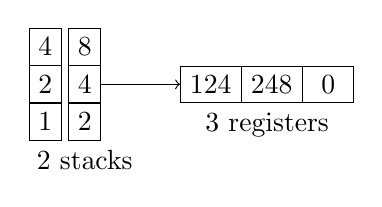
\begin{tikzpicture}[stack/.style={rectangle split, rectangle split parts=#1,draw}]

% two stacks
\node (pds_0)[stack=3]  {
\nodepart{one}4
\nodepart{two}2
\nodepart{three}1
};
\node (pds_1)[label=below:2 stacks, stack=3] at (0.5, 0){
\nodepart{one}8
\nodepart{two}4
\nodepart{three}2
};

% 3 registers
\node (reg) [label=below:3 registers, draw,rectangle split, rectangle split horizontal,rectangle split parts=3, right = of pds_1]{
\nodepart{one}124
\nodepart{two}248
\nodepart{three}\ 0 \
};

\draw [->] (pds_1) edge (reg);
\end{tikzpicture}
\captionof{figure}{From 2-PDS to 3-register}
\end{tightcenter}

Each stack is encoded as a decimal number where the top element of the stack is represent by the least significant digit. This way the top element can be easily identified using the modulo 10 operation. Its removal corresponds to a division by 10, pushing a number $k$ to the stack corresponds to multiplication by 10 followed by an addition of $k$. The $n +1$ register is needed since multiplication and division require an auxiliary register. If the stack alphabet is different from $\{1,\ldots,9\}$ a different base is needed.

$n$-register $\to$ $2$-register:\\
The first register holds the encoding of the $n$ registers of the original machine as a product of the first $n$ prime numbers, with the register values stored as their exponents: \\

\begin{tightcenter}
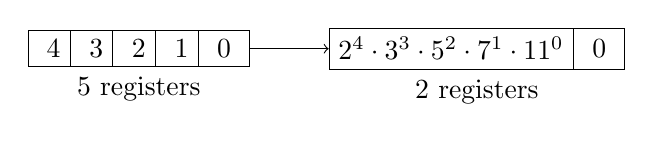
\begin{tikzpicture}[stack/.style={rectangle split, rectangle split parts=#1,draw}]

% 3 registers
\node (reg_0) [label=below:5 registers, draw,rectangle split, rectangle split horizontal,rectangle split parts=5]{
\nodepart{one}\ 4 \
\nodepart{two}\ 3 \
\nodepart{three}\ 2 \
\nodepart{four}\ 1 \
\nodepart{five}\ 0 \
};

% two registers
\node (reg_1) [label=below:2 registers, draw,rectangle split, rectangle split horizontal,rectangle split parts=2, right = of reg_0]{
\nodepart{one}$2^4 \cdot 3^3 \cdot 5^2 \cdot 7^1 \cdot 11^0$
\nodepart{two}\ 0 \
};

\draw [->] (reg_0) edge (reg_1);
\end{tikzpicture}
\captionof{figure}{From 5-register to 2-register}
\end{tightcenter}

The second register is again just a helper register for multiplication, division and storing division remainder. Checking whether register $i \in [1\ldots n]$ is equal to 0 corresponds to dividing our encoding by the ith prime number. If the division has a remainder the ith register value must have been 0. Indeed the encoding in our example $(2^4 \cdot 3^3 \cdot 5^2 \cdot 7^1 \cdot 11^0)$ is dividable by all prime numbers up to 7 but has a remainder of 1 when divided by 11.
\end{proof}
\subsection{Data Words}
\begin{defi}{Data Words}
    A \emph{data word} is a word $w \in \Sigma^\ast$, $\abs{w} = n$ together with \emph{data} for each position, represented by a function $d : \Set{1,\ldots,n} \to \nat$.
\end{defi}

We extend logic to data-words in the following way:

In addition to the usual parts of FO/MSO over words, we add relations
\begin{itemize}
    \item $d(x) = 0$
    \item $d(x) = d(y)$, $d(x) < d(y)$, $d(x) \le d(y)$
    \item $d(x) = d(y) + 1$
\end{itemize}
for terms $x,y$.

Satisfiability for FO-sentences modulo data-words (given a sentence $\varphi$, does there exist a data-word $w,d$ satisfying it?) is undecidable.
\begin{proof} We can construct an FO-sentence describing valid, terminating computations of a $2$-register machine. Thus we reduce the halting problem of $2$-register machines to the satisfiability of FO-sentences over data-words.

    This construction uses as an alphabet the line numbers of the register machine's program, together with a \emph{padding symbol} $\#$. A word describes the sequence of line numbers in the order they were visited with $\#$ following each line number. Pairs of data cells represent the two register values: \\
    
\begin{tightcenter}
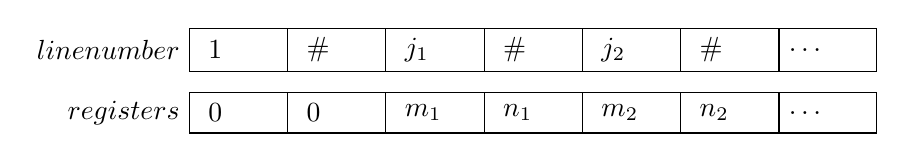
\begin{tikzpicture}[stack/.style={ text width=3cm,rectangle split, rectangle split parts=#1,draw}]

% word
\node (word) [label=left: $line number$, draw,rectangle split, rectangle split horizontal,rectangle split parts=7, text width=1cm] {
\nodepart{one}\ $1$ \ 
\nodepart{two}\ $\#$ \ 
\nodepart{three}\ $j_1$ \ 
\nodepart{four}\ $\#$ \ 
\nodepart{five}\ $j_2$ \ 
\nodepart{six}\ $\#$ \ 
\nodepart{seven}\ldots
};

% data
\node (data) [label=left: $registers$, draw,rectangle split, rectangle split horizontal,rectangle split parts=7, text width=1cm] at (0, -0.8){
\nodepart{one}\ $0$ \ 
\nodepart{two}\ $0$ \ 
\nodepart{three}\ $m_1$ \ 
\nodepart{four}\ $n_1$ \ 
\nodepart{five}\ $m_2$ \ 
\nodepart{six}\ $n_2$ \ 
\nodepart{seven}\ldots
};

\end{tikzpicture}

\captionof{figure}{Potentially valid data-word for a 2-register machine}
\end{tightcenter}

    Our conjunction of FO-formulas asserts that we are initially in line 1 and both registers are equal to 0. Furthermore the word contains the line number of the $stop$-instruction at some point. The register machine's instructions are translated to FO-formula so that line numbers and register values of the data word change as expected from the simulated instructions: We are axiomatizing valid computations/runs of the given register machine.
\end{proof}

\section{Communication via FIFO Channels}

\begin{halfboxl}
\vspace{-\baselineskip}
In an attempt to model communicating processes, we introduce the notion of \emph{message passing automata}, wherein multiple automata can communicate messages of a finite alphabet via queues.

However, this model is too powerful to be effectively analysed: The simple reachability problem for message passing automata is undecidable even when restricted to a single automaton with a queue to itself.

\begin{proof}
One can simulate the run of a turing machine, using the queue to hold the contents of the tape.
\end{proof}
\end{halfboxl}%
\begin{halfboxr}
\vspace{-\baselineskip}
\begin{defi}{Message Passing Automaton}
    A \emph{message passing automaton} is a structure $(CN, \Gamma, \mathcal{A}_1, \ldots, \mathcal{A}_n)$ with
    \begin{itemize}[leftmargin=1.0em]
        \item set of channels $CN \subseteq \Set{1,\ldots,n}^2$ \\
        {\footnotesize{}\textcolor{darkgray}{$(i, j)$ is the channel $\A_i$ \emph{writes} and $A_j$ \emph{reads} from}}
            \smallskip
        \item message alphabet $\Gamma$
        \item automata $\mathcal{A}_i = (Q_i, \Sigma_i, q_{0i}, \Delta_i, F_i)$ with transitions of the form
        \begin{itemize}[leftmargin=1.0em]
            \item $(p, a, q)$ with $p,q \in Q_i$, $a \in \Sigma_i$
            \item $(p, m!j, q)$ with $p,q \in Q_i$, $m \in \Gamma$ and $(i,j) \in CN$   \\
            (Write $m$ to channel $(i,j)$) \\
        {\footnotesize{}\textcolor{darkgray}{Automata write from the left.}}
            \smallskip
            \item $(p, m?j, q)$ with $p,q \in Q_i$, $m \in \Gamma$ and $(j,i) \in CN$   \\
            (If $m$ is the first letter of channel $(j,i)$, remove it and go to state $q$) \\
        {\footnotesize{}\textcolor{darkgray}{Automata read from the right.}}
            \smallskip
        \end{itemize}
    \end{itemize}
    Configurations for message passing automata contain the states of each automaton as well as the contents of each channel.
\end{defi}
\end{halfboxr}

\end{document}
